\section{}

\subsection{}
A Pb–$60$ at$\%$ Sn alloy was slowly cooled from 380°C to 50°C. Calculate the volume fraction of the primary phase at $50°$C.

\begin{figure}[h]
 \centering
 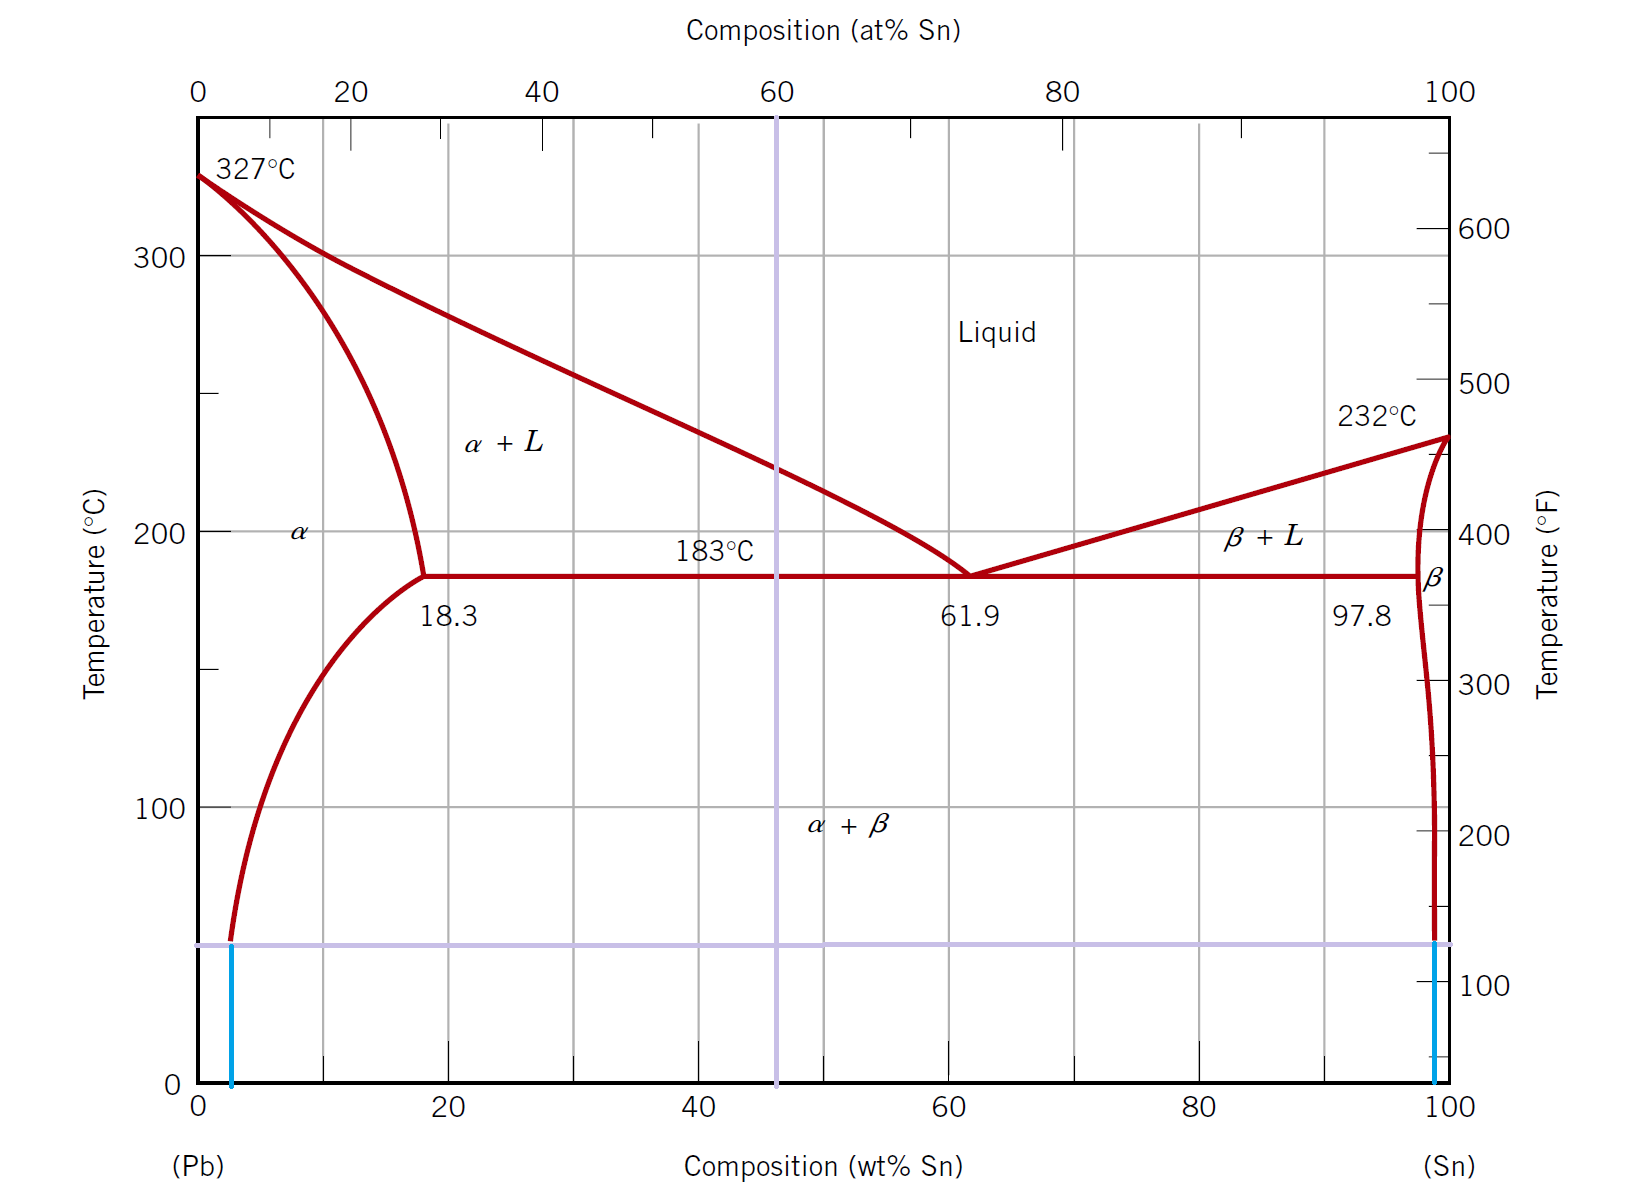
\includegraphics[width=0.8\textwidth]{graficas/diagrama.png}}
 \caption{a) Diffusion coefficient $D$ ($m^2/s)$ as a function of temperature $T$ (K) and b) logarithm of the diffusion coefficient $ln(D)$ as a function of the inverse of the temperature $1/T$ ($K^{-1}$) for self-diffusion systems. \\
 \textit{Source: Data from \citep{kakusan}, visualization by the author (code available at \citep{}).}}
 \label{}
\end{figure}

\subsection{}
A Pb–$25$ at$\%$ Sn alloy was slowly cooled from 380°C to 50°C. Ideally, Sn phase is expected to precipitate within Pb-phase grains, but in reality, a eutectic structure appeared. Assuming there were no experimental issues such as weighing errors, discuss the reason why this phenomenon occurred.